توضیح کلی راه حل

\subsection*{1.}
\subsubsection*{الف}

توضیحات

\subsubsection*{ب}

توضیحات

\subsection*{2.}
\subsubsection*{الف}
این عبارت منظم، تمامی رشته‌های متشکل از 0 و 1 را می‌پذیرد. پس DFA آن به این صورت خواهد بود:

\begin{figure}[htbp]
	\centering
	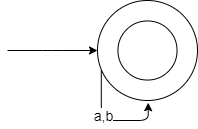
\includegraphics[width=0.20\textwidth]{q3s2p1.png}
\end{figure}



\subsubsection*{ب}
با توجه به عبارت منظم داده شده، DFA را رسم می‌کنیم:
\begin{figure}[htbp]
	\centering
	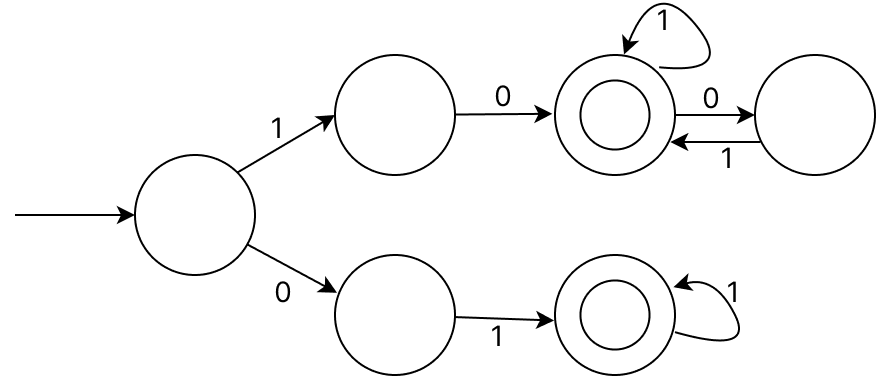
\includegraphics[width=0.55\textwidth]{q3s2p2.png}
\end{figure}

\subsection*{3.}
\subsubsection*{الف}
برای رسم DFA از روی NFA لازم است از مجموعه ${\LARGE \epsilon} - closure$ مربوط به هر State استفاده کنیم:

\setLTR

${\LARGE \epsilon} - closure(A)= \left\{A,C\right\}$ \hspace{1em} ${\LARGE \epsilon} - closure(B)= \left\{B\right\}$ 

${\LARGE \epsilon} - closure(C)=\left\{C\right\}$  \hspace{1.9em}  ${\LARGE \epsilon} - closure(D)= \left\{D\right\}$ 

\setRTL

\begin{figure}[htbp]
	\centering
	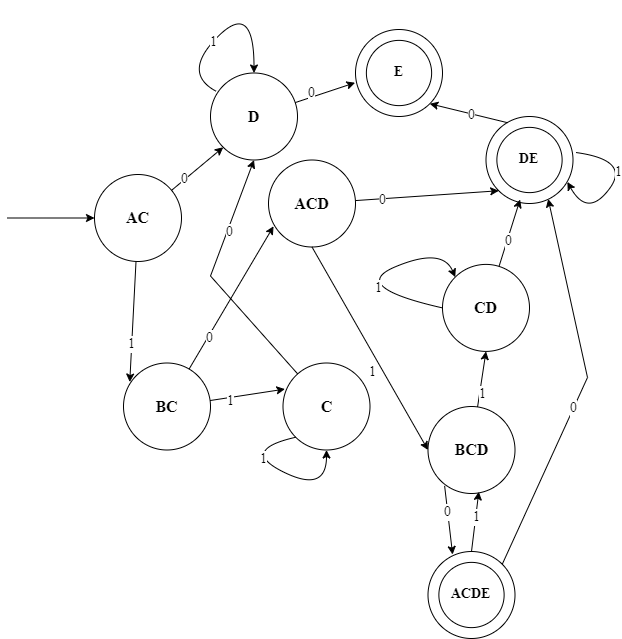
\includegraphics[width=0.55\textwidth]{q3s3p1.png}
\end{figure}

\subsubsection*{ب}

